% =============================================================================
% template.tex — Template LaTeX para bookdown/ufprdown
% Usa a classe ppginf.cls (oficial PPGInf/UFPR). O arquivo .cls NÃO deve ser
% modificado, pois contém os padrões de formatação da UFPR.
% =============================================================================

% ─── CONFIGURAÇÃO DA CLASSE ───────────────────────────────────────────
% O pacote 'comment' é carregado em setup/packages.tex (necessário para os
% ambientes comment/endcomment da ppginf.cls no modo defesa).
$if(final_mode)$
\documentclass[final,oneside,english,brazilian]{ppginf}
$else$
\documentclass[defesa,oneside,english,brazilian]{ppginf}
$endif$

% ─── PACOTES ────────────────────────────────────────────────────────────────
% =============================================================================
% packages.tex — Pacotes e configurações globais para ufprdown
% Baseado no packages.tex original do template PPGInf/UFPR
% =============================================================================

% ── Codificação e fontes ─────────────────────────────────────────────────────
\usepackage[utf8]{inputenc}
\usepackage[T1]{fontenc}

\usepackage{ifthen}
\usepackage{courier}                    % Verbatim, Listings, etc

% ── Matemática ───────────────────────────────────────────────────────────────
\usepackage{amsmath}
\usepackage{amsfonts}
\usepackage{amssymb}
\usepackage{amsthm}
\usepackage{bm}                         % negrito matemático (\bm{})
\usepackage{xparse}                     % para \NewDocumentCommand (citeproc)

% Teoremas (desativado porque o bookdown usa amsthm e já define seus próprios labels
% baseados no bloco 'language:' do _bookdown.yml. Se definirmos aqui, dá erro
% de 'command \theorem already defined').

% Operadores matemáticos
\DeclareMathOperator{\E}{\mathbb{E}}
\DeclareMathOperator{\Var}{Var}
\DeclareMathOperator{\Cov}{Cov}
\DeclareMathOperator{\logit}{logit}
\DeclareMathOperator{\diag}{diag}

% ── Figuras ──────────────────────────────────────────────────────────────────
\usepackage{graphicx}
\usepackage[labelformat=simple]{subcaption}
\renewcommand\thesubfigure{(\alph{subfigure})}

% ── Tabelas ──────────────────────────────────────────────────────────────────
\usepackage{booktabs}                   % \toprule, \midrule, \bottomrule
\usepackage{longtable}                  % tabelas multi-páginas
\usepackage{multirow}                   % células mescladas
\usepackage{array}                      % extensões para tabelas

% ── Código-fonte ─────────────────────────────────────────────────────────────
\usepackage{listings}
\usepackage{xcolor}

\definecolor{codegreen}{rgb}{0,0.6,0}
\definecolor{codegray}{rgb}{0.5,0.5,0.5}
\definecolor{codepurple}{rgb}{0.58,0,0.82}
\definecolor{backcolour}{rgb}{0.97,0.97,0.95}

\lstdefinestyle{thesis-code}{
    backgroundcolor=\color{backcolour},
    commentstyle=\color{codegreen},
    keywordstyle=\color{magenta},
    numberstyle=\tiny\color{codegray},
    stringstyle=\color{codepurple},
    basicstyle=\ttfamily\footnotesize,
    breaklines=true,
    captionpos=b,
    keepspaces=true,
    numbers=left,
    numbersep=5pt,
    frame=single,
    columns=flexible,
    mathescape=true,
    inputencoding=utf8,
    extendedchars=true,
}
\lstset{style=thesis-code}

% Suporte a caracteres acentuados em listings (do template original)
\lstset{literate={á}{{\'a}}1  {ã}{{\~a}}1 {à}{{\`a}}1 {â}{{\^a}}1
                 {Á}{{\'A}}1  {Ã}{{\~A}}1 {À}{{\`A}}1 {Â}{{\^A}}1
                 {é}{{\'e}}1  {ê}{{\^e}}1 {É}{{\'E}}1  {Ê}{{\^E}}1
                 {í}{{\'\i}}1 {Í}{{\'I}}1
                 {ó}{{\'o}}1  {õ}{{\~o}}1 {ô}{{\^o}}1
                 {Ó}{{\'O}}1  {Õ}{{\~O}}1 {Ô}{{\^O}}1
                 {ú}{{\'u}}1  {Ú}{{\'U}}1
                 {ç}{{\c{c}}}1 {Ç}{{\c{C}}}1 }

% ── Algoritmos ───────────────────────────────────────────────────────────────
\usepackage{algorithm,algorithmic}
\floatname{algorithm}{Algoritmo}
\renewcommand{\algorithmiccomment}[1]{~~~// #1}

% ── Bibliografia ─────────────────────────────────────────────────────────────
% As citações são processadas pelo pandoc citeproc (pandoc >= 3.x).
% O estilo de citação é definido pelo arquivo CSL no YAML (csl: csl/apa.csl).

% ── Pacotes diversos ─────────────────────────────────────────────────────────
\usepackage{alltt}                      % verbatim melhorado
\usepackage{lipsum}                     % texto aleatório (p/ exemplos)
\usepackage[final]{pdfpages}            % inclusão de páginas em PDF
\usepackage{rotating}                   % rotação de tabelas/figuras

% ── Quadros (UFPR) ──────────────────────────────────────────────────────────
\usepackage{float}
\newfloat{quadro}{htbp}{loq}[chapter]
\floatname{quadro}{Quadro}
\newcommand{\listofquadros}{\listof{quadro}{Lista de Quadros}}

% ── Comandos personalizados ──────────────────────────────────────────────────
\newcommand{\bbeta}{\bm{\beta}}
\newcommand{\bgamma}{\bm{\gamma}}
\newcommand{\btheta}{\bm{\theta}}
\newcommand{\bSigma}{\bm{\Sigma}}
\newcommand{\TODO}[1]{\textcolor{red}{\textbf{[TODO: #1]}}}

% Atalhos úteis para centralização e fonte (notas de autor)
\newcommand{\bcenter}{\begin{center}}
\newcommand{\ecenter}{\end{center}}

% ── Anexo ───────────────────────────────────────────────% Definição de \anexo (similar ao \appendix da ppginf.cls)
\makeatletter
\newcommand{\@taganexo}{ANEXO}
\newcommand{\anexo@chapter}[1]{%
  \refstepcounter{chapter}%
  \orig@chapter*{\@taganexo\ \@Alph\c@chapter\enskip -- \enskip\MakeUppercase{#1}}%
  \addcontentsline{toc}{chapter}{\@taganexo\ \@Alph\c@chapter\enskip -- \enskip\uppercase{#1}}}%
\newcommand{\anexo}{%
  \setcounter{chapter}{0}%
  \renewcommand{\thechapter}{\@Alph\c@chapter}%
  \let\chapter\anexo@chapter%
}
\makeatother


% ─── FONTES (Times New Roman ou Arial) ──────────────────────────────────────
$if(font-family)$
\ifthenelse{\equal{$font-family$}{Arial}}{
  \usepackage{helvet}
  \renewcommand{\familydefault}{\sfdefault}
}{
  \usepackage{mathptmx}
}
$else$
\usepackage{mathptmx}
$endif$

$if(highlighting-macros)$
$highlighting-macros$
$endif$

% Comandos auxiliares para bookdown/pandoc
\providecommand{\tightlist}{\setlength{\itemsep}{0pt}\setlength{\parskip}{0pt}}

% Compatibilidade com pandoc >= 3.2.1 (Undefined control sequence \pandocbounded)
\providecommand{\pandocbounded}[1]{#1}

% Compatibilidade com pandoc citeproc (pandoc >= 3.x)
\NewDocumentCommand\citeproctext{}{}
\NewDocumentCommand\citeproc{mm}{%
  \begingroup\def\citeproctext{#2}\cite{#1}\endgroup}
\makeatletter
 % allow citations to break across lines
 \let\@cite@ofmt\@firstofone
 % avoid brackets around text for \cite:
 \def\@biblabel#1{}
 \def\@cite#1#2{{#1\if@tempswa , #2\fi}}
\makeatother
\newlength{\cslhangindent}
\setlength{\cslhangindent}{1.5em}
\newlength{\csllabelwidth}
\setlength{\csllabelwidth}{3em}
% CSLReferences: pandoc 3.x emite \bibitem[\citeproctext]{...} dentro deste ambiente.
% \bibitem usa \item internamente e EXIGE thebibliography. Usamos thebibliography
% como base para garantir compatibilidade. O título (REFER\^ENCIAS / REFERENCES)
% é gerado automaticamente pelo thebibliography via \bibname, e o tocbibind
% adiciona-o ao sumário. Não repita o título no Rmd.
\ifdefined\CSLReferences
\else
\newenvironment{CSLReferences}[2]{%
  \begin{thebibliography}{MMMMM}%
}{%
  \end{thebibliography}%
}
\fi

$for(header-includes)$
$header-includes$
$endfor$

\makeatletter
% Títulos estruturais: SEMPRE em maiúsculo por norma ABNT/UFPR,
% independente de element_names_up (que controla apenas prefixos de legenda).
  \def\@listacronyms{LISTA DE SIGLAS}
  \def\@listsymbols{LISTA DE S\'IMBOLOS}
  \def\@chapthanks{AGRADECIMENTOS}
  \def\@tagappendix{AP\^ENDICE}
  \def\@taganexo{ANEXO}
\makeatother

\AtBeginDocument{
% Títulos estruturais: SEMPRE em maiúsculo (norma ABNT/UFPR)
  \renewcommand{\listfigurename}{LISTA DE FIGURAS}
  \renewcommand{\listtablename}{LISTA DE TABELAS}
  \renewcommand{\proofname}{DEMONSTRA\c{C}\~AO}
  \renewcommand{\appendixname}{AP\^ENDICE}
  \renewcommand{\contentsname}{SUM\'ARIO}
  \renewcommand{\bibname}{REFER\^ENCIAS}
  \renewcommand{\listofquadros}{\listof{quadro}{LISTA DE QUADROS}}
% Prefixos de legenda: controlados por element_names_up
$if(element_names_up)$
  \renewcommand{\figurename}{FIGURA}
  \renewcommand{\tablename}{TABELA}
  \floatname{quadro}{QUADRO}
$else$
  \renewcommand{\figurename}{Figura}
  \renewcommand{\tablename}{Tabela}
  \floatname{quadro}{Quadro}
$endif$
}

\AtBeginDocument{
$if(element_names_up)$
\DeclareCaptionLabelFormat{upper}{\MakeUppercase{#1} #2}
\captionsetup{labelformat=upper}
$endif$
}


$if(fig_caption_position)$
$if(fig_caption_position_bottom)$
\floatstyle{plain}
$else$
\floatstyle{plaintop}
$endif$
\restylefloat{figure}
\restylefloat{table}
\restylefloat{quadro}
$endif$

% ─── INÍCIO DO DOCUMENTO ────────────────────────────────────────────────────
\begin{document}

% ─── METADADOS ──────────────────────────────────────────────────────────────

\title{$title$}

$if(palavras-chave)$
\pchave{$palavras-chave$}
$endif$
$if(keywords)$
\keyword{$keywords$}
$endif$

\author{$author$}
\advisor{$advisor$}
$if(coadvisor)$
\coadvisor{$coadvisor$}
$endif$

$if(institution)$
\instit{$inst_short$}{$institution$}
$else$
\instit{UFPR}{Universidade Federal do Paraná}
$endif$

$if(field)$
\field{$field$}
$else$
\field{Ciência da Computação}
$endif$

\date{$date_year$}

$if(local)$
\local{$local$}
$else$
\local{Curitiba PR}
$endif$

$if(coverimage)$
\coverimage{$coverimage$}
$endif$

$if(descr)$
\descr{$descr$}
$else$
\descr{$doc_type$ apresentada como requisito parcial à obtenção do grau de $degree$ no $course$, da $institution$.}
$endif$

% =============================================================================
% PARTE PRÉ-TEXTUAL
% =============================================================================

\frontmatter
\pagestyle{frontmatter}

\titlepage

% Ficha catalográfica (só na versão final)
$if(final_mode)$
\begin{ficha}
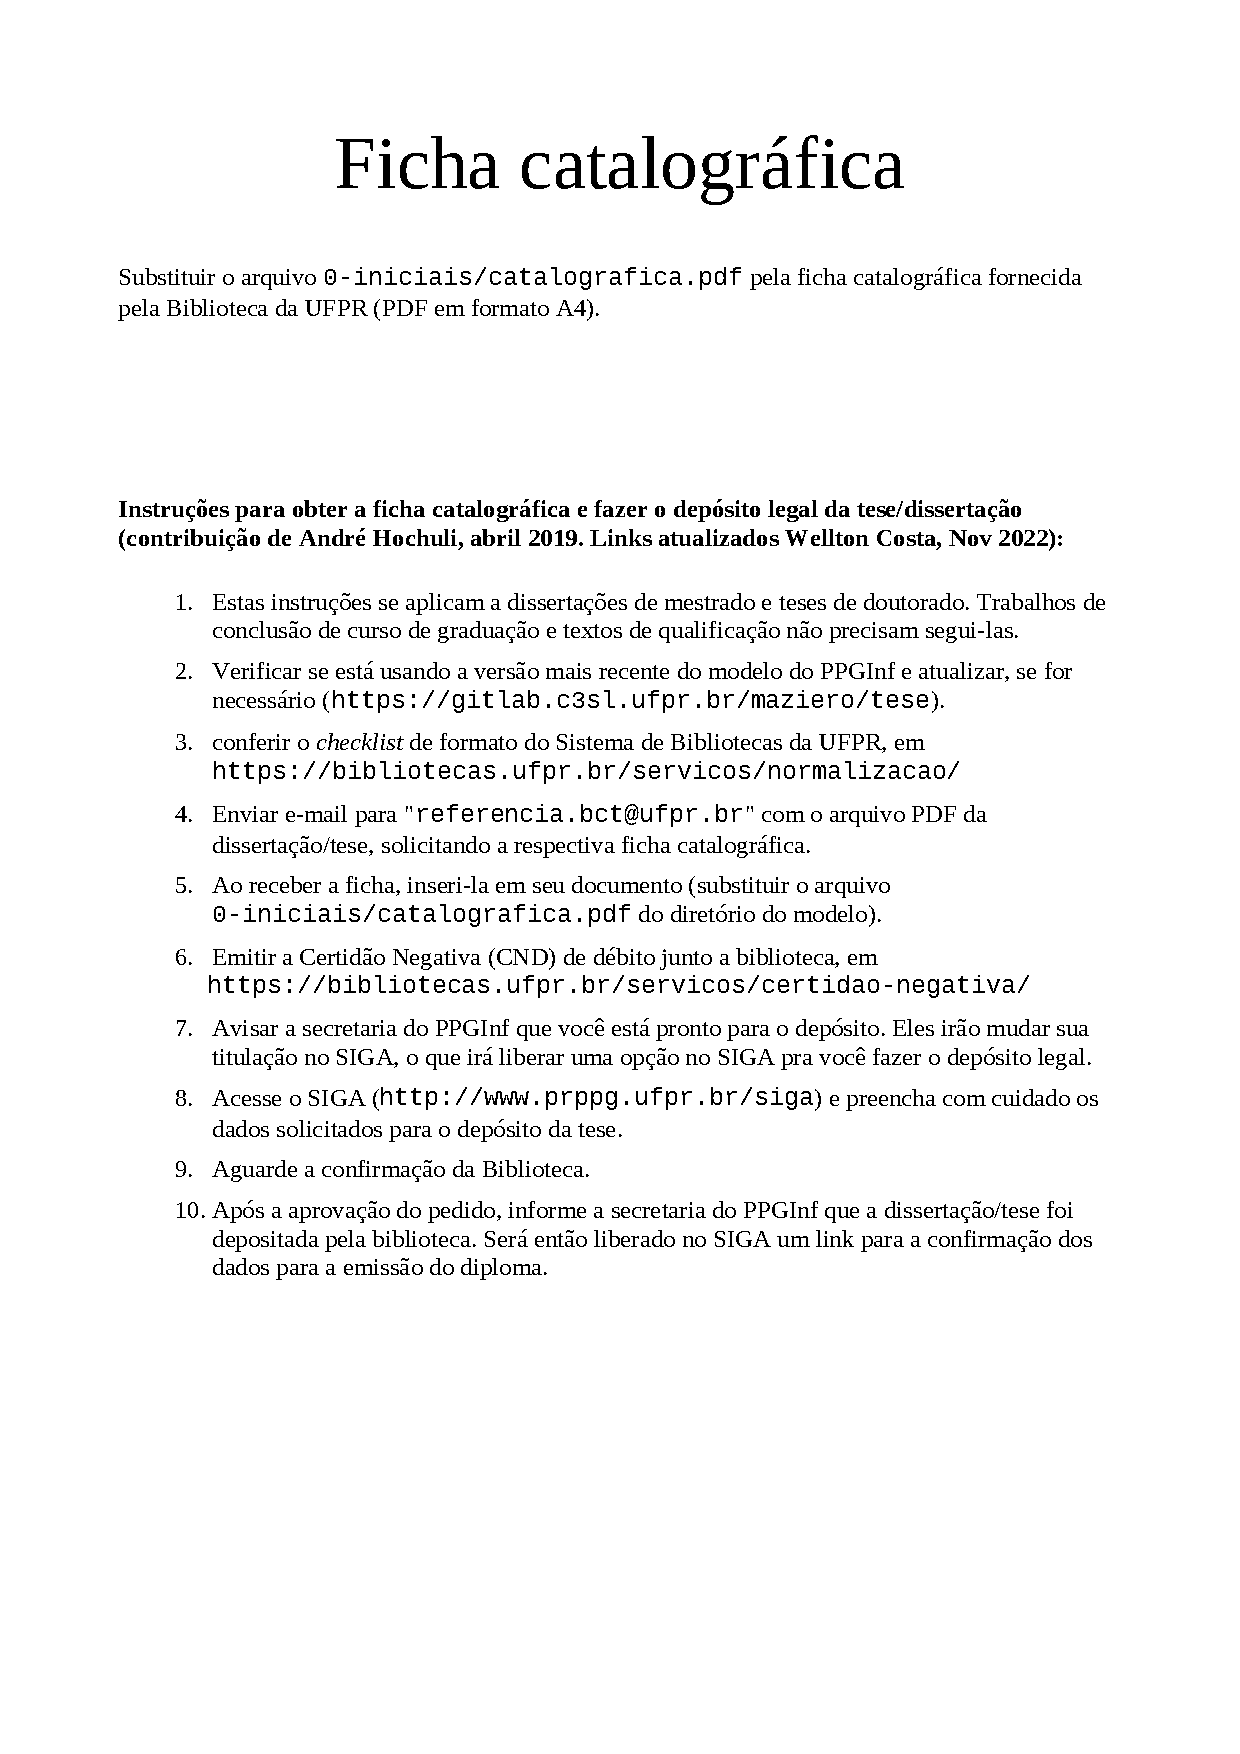
\includepdf[noautoscale]{Ficha_Catalografica.pdf}
\end{ficha}
$endif$

% Folha de aprovação (só na versão final)
$if(final_mode)$
\begin{aprovacao}
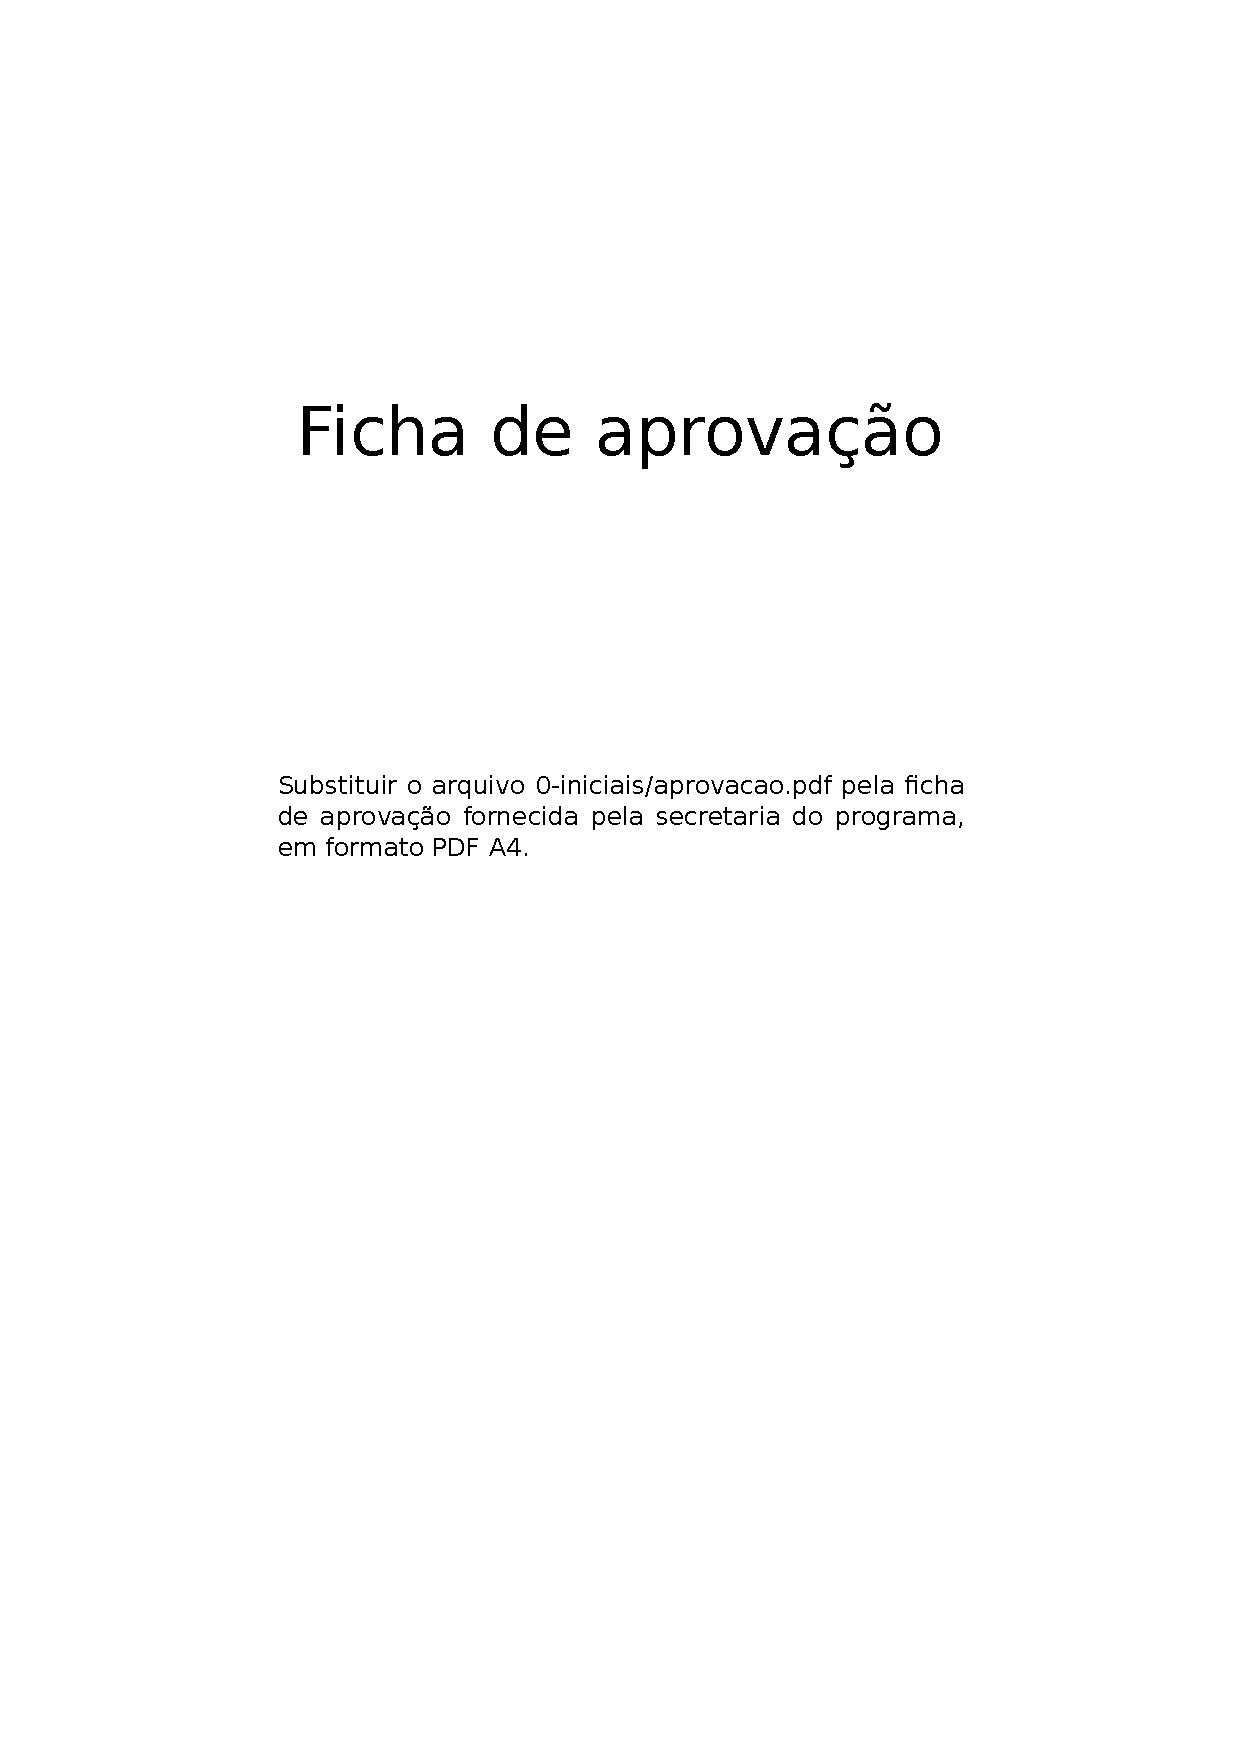
\includepdf[noautoscale]{aprovacao.pdf}
\end{aprovacao}
$endif$

% Dedicatória (só na versão final)
$if(final_mode)$
$if(dedication)$
\begin{dedica}
$dedication$
\end{dedica}
$endif$
$endif$

% Agradecimentos (só na versão final)
$if(final_mode)$
$if(thanks)$
\begin{agradece}
$thanks$
\end{agradece}
$endif$
$endif$

% Resumo (palavras-chave são inseridas automaticamente pelo ppginf.cls
% através dos comandos \pchave{} e \keyword{} definidos acima)
$if(abstract)$
\begin{resumo}
$abstract$
\end{resumo}
$endif$

% Abstract
$if(foreignabstract)$
\begin{abstract}
$foreignabstract$
\end{abstract}
$endif$

% Listas
\listoffigures
\clearpage
\listoftables
\clearpage
\listofquadros
%=====================================================
% Lista de acrônimos (siglas e abreviações)
%=====================================================

\begin{listaacron}

\begin{longtable}[l]{p{0.2\linewidth}p{0.7\linewidth}}
AGHQ  & \textit{Adaptive Gauss-Hermite Quadrature} (Quadratura de Gauss-Hermite Adaptativa)\\
AIC   & \textit{Akaike Information Criterion} (Critério de Informação de Akaike)\\
BIC   & \textit{Bayesian Information Criterion} (Critério de Informação Bayesiano)\\
CRAN  & \textit{Comprehensive R Archive Network}\\
EQM   & Erro Quadrático Médio\\
GLM   & \textit{Generalized Linear Model} (Modelo Linear Generalizado)\\
GLMM  & \textit{Generalized Linear Mixed Model} (Modelo Linear Generalizado Misto)\\
IC    & Intervalo de Confiança\\
LA    & \textit{Laplace Approximation} (Aproximação de Laplace)\\
MV    & Máxima Verossimilhança\\
NRS   & \textit{Numerical Rating Scale} (Escala de Avaliação Numérica)\\
PPGMNE & Programa de Pós-Graduação em Métodos Numéricos em Engenharia\\
QMC   & \textit{Quasi-Monte Carlo}\\
UFPR  & Universidade Federal do Paraná\\
VAS   & \textit{Visual Analog Scale} (Escala Visual Analógica)\\
\end{longtable}

\end{listaacron}

%=====================================================
% Lista de símbolos
%=====================================================

\begin{listasimb}

\begin{longtable}[l]{p{0.2\linewidth}p{0.7\linewidth}}
$y_{ij}$       & Resposta observada do $j$-ésimo indivíduo no $i$-ésimo grupo\\
$\mu_{ij}$     & Média condicional da distribuição beta para a observação $ij$\\
$\phi_{ij}$    & Parâmetro de precisão da distribuição beta para a observação $ij$\\
$\sigma^2$     & Variância\\
$\bm{\beta}$   & Vetor de coeficientes de regressão (efeitos fixos para $\mu$)\\
$\bm{\gamma}$  & Vetor de coeficientes de regressão (efeitos fixos para $\phi$)\\
$\bm{b}_i$     & Vetor de efeitos aleatórios para o $i$-ésimo grupo\\
$\bm{D}$       & Matriz de covariância dos efeitos aleatórios\\
$g(\cdot)$     & Função de ligação para a média\\
$\ell(\cdot)$  & Função de log-verossimilhança\\
$n$            & Número total de observações\\
$q$            & Dimensão do vetor de efeitos aleatórios\\
$p$            & Número de parâmetros de efeitos fixos\\
\end{longtable}

\end{listasimb}

\tableofcontents

% =============================================================================
% CORPO DO DOCUMENTO
% =============================================================================

\mainmatter
\pagestyle{mainmatter}

$body$

% =============================================================================
% REFERÊNCIAS (processadas pelo pandoc citeproc)
% =============================================================================

$for(include-after)$
$include-after$
$endfor$

% =============================================================================

\end{document}
